\documentclass[conference]{IEEEtran}
% Add the compsoc option for Computer Society conferences.
%
% If IEEEtran.cls has not been installed into the LaTeX system files,
% manually specify the path to it like:
% \documentclass[conference]{../sty/IEEEtran}

\usepackage{listings}
\usepackage{algorithm}
\usepackage{algorithmic}
\usepackage{amsmath}
\usepackage{pgf}
\usepackage{url}
\usepackage{tikz}
\usepackage{pict2e}
\usepackage{flushend}
\usepackage{pifont}
\usetikzlibrary{calc}
\usetikzlibrary{shapes}

\usepackage{fixltx2e}
% fixltx2e, the successor to the earlier fix2col.sty, was written by
% Frank Mittelbach and David Carlisle. This package corrects a few problems
% in the LaTeX2e kernel, the most notable of which is that in current
% LaTeX2e releases, the ordering of single and double column floats is not
% guaranteed to be preserved. Thus, an unpatched LaTeX2e can allow a
% single column figure to be placed prior to an earlier double column
% figure. The latest version and documentation can be found at:
% http://www.ctan.org/tex-archive/macros/latex/base/

\newcommand{\comment}[1]{{\sf\color{blue}(#1)}}
\newcommand{\ignore}[1]{}
\newcommand\figref[1]{Figure~\ref{#1}}
\newcommand\secref[1]{Section~\ref{#1}}

% correct bad hyphenation here
\hyphenation{op-tical net-works semi-conduc-tor}

\begin{document}
\title{Conditional Data Flow Analysis}


\author{\IEEEauthorblockN{Elena Sherman}
\IEEEauthorblockA{Department of Computer Science and Engineering\\
University of Nebraska - Lincoln\\
Lincoln, Nebraska 68588-015\\
Email: esherman@cse.unl.edu}
\and
\IEEEauthorblockN{Matthew B. Dwyer}
\IEEEauthorblockA{Department of Computer Science and Engineering\\
University of Nebraska - Lincoln\\
Lincoln, Nebraska 68588-015\\
Email: dwyer@cse.unl.edu}
}

\maketitle

\begin{abstract}
The abstract goes here.
\end{abstract}

\section{Introduction}
\label{section:introduction}
%Type of systems suitable for SA.
The degree to which a software must satisfy its requirements depends on the criticality of the software. An undetected fault in critical software may result in significant financial losses or human fatalities, e.g., a fault in a flight control system. Thus, the degree of the conformance, i.e., an adequacy criterion,  for critical software is set at the highest level -- software must comply with its requirements on all possible inputs. Yet, for the majority of applications adequacy criteria are more relaxed, e.g., to be $85\%$ statement adequate, a property must hold on a set of inputs that executes $85\%$ of the application's statements. 

To accommodate these different levels of compliance, software engineers have developed various techniques best suitable for a specific criterion. Mainly these techniques are classified into dynamic and static analyses. Dynamic analysis, such as testing, verifies that a program is adequate by executing it. This approach is widely used for non-critical software that uses weaker adequacy criteria. Employing testing to check a program's conformance on all inputs is usually intractable. Static analysis checks the conformance of a program to its property by analyzing the program code, i.e., without executing it. This compile-time determination allows static analysis to consider all possible program behaviors, which is suitable for checking program conformance to its properties at the highest level. Hence, static analysis is a key technique for verifying critical systems.
 
%Not enough precise SA. False positives.
The power of static analysis to consider all program behaviors follows from its ability to safely approximate program behaviors by abstracting the concrete domain of program variables and the programming language semantics. But at the same time because of its over-approximating nature, static analysis may identify some property violations as uncertain. The reason for this uncertainty is that a static analysis cannot tell if a violation happens on a feasible or an infeasible program behavior. This inconclusiveness is unacceptable for critical system and thus each potential violation must be examined further. An automatic solution to the elimination of false positive violations is to increase the precision of a static analysis, i.e., improve the analysis so it considers fewer infeasible behaviors.

%SA can be make arbitrary precise by either making its domain finer (C\&C 77) or combining different analyses together (C\&C 79). Scalability issues.
%Scalability and precision as two opposing properties of SA. Ideally good scalability and good precision together. Two approach to maintain both.
One way to improve the precision of a static analysis is to refine its abstract domain and program semantics interpretation which is always theoretically possible~\cite{Cousot:1977}, or to combine different static analyses in a suitable manner as discussed in~\cite{Cousot:1979}. Besides the laborious effort of redesigning a static analysis or combining two of them together, the resulting analysis usually becomes expensive in terms of time and memory consumption which makes it inapplicable to large applications. Thus precision and scalability of a static analysis work against each other. When a static analysis has a high precision generally it is not scalable and conversely when a static analysis is scalable its precision typically suffers. The literature suggests two complementary ideas for approaching this dilemma.\\
One approach focuses on making a precise static analysis scalable by partitioning a large program into modules like procedures and classes, and allowing the analysis to examine each partition independently. Next, the analyzed information of each module is composed together to obtain the result of  the whole program analysis. In the literature~\cite{Cousot:2002, Ballabriga:2007} this method is referred to as {\em partial static analysis}.\\
%Can put Corina's there if it said that it can only handle couple modules
%Conditional analyses. 3 papers. Assumes some conditions holds and another analyses should verify that these conditions holds
Another approach concentrates on improving the precision of a scalable analysis by permitting the analysis to explore only those program states for which it is adequately precise, i.e., able to provide definitive result. In the literature~\cite{Naik:POPL07,Conway:SAS08, Beyer:Tech11} this approach is called {\em conditional static analysis} since the permitted states are described by a condition $\theta$. In this framework an analysis verifies a program under some assumptions, i.e., there is no null pointer exception in the program. Next, another analysis attempts to prove these assumptions by either showing that the states which do not satisfy $\theta$ are not reachable or do not lead to property violations. In the previous work the condition $\theta$ either determined from the analysis design~\cite{Naik:POPL07,Conway:SAS08} when $\theta$ is applicable to all program states or determined during program analysis execution~\cite{Beyer:Tech11} when $\theta$ is composed from the conditions assumed to be held for a certain set of states.\\
%State briefly what has been done in the previous work of conditional model checker and conditional soundness and what we are doing different there. Write related work first?
%Our work explores conditional data-flow analyses. What challenges or what has been accomplished.
Our work focuses on the latter approach applied to data-flow analysis, i.e., conditional data-flow analysis. Unlike the cases presented in the previous work, data-flow analysis cannot determine a priori or during its execution the conditions under which it is able to verify a program to its best abilities. Moreover, data-flow analysis has two alternative ways for expressing $\theta$. The main goal of our work is to explore different approaches in $\theta$ encoding for data-flow analysis so that a scalable analysis is able to optimize its result. In the next section we illustrate the concept of conditional data-flow analysis, different encodings for $\theta$ and their effect. In the next section we also present our research questions and the outline for the rest of the paper.
%The main difference is that condition is unknown a priori . Condition can be specified in multiple ways.

\section{Overview}
\label{section:overview}
%Here we want to illustrate the reasons why conditional support in existing data flow analyses is too restricted and why support for model checking is not appropriate.

%We should do it by way of examples and introduce the concepts and advantages of our proposed approaches.

%Show a general analysis.\\
Before introducing conditional data-flow analysis we would like to start with an example of a traditional data-flow analysis. Data-flow analysis calculates some information for each point in a program based on the program structure and  the language semantics. The calculated facts then later used to reason about program properties. One type of property that we consider in this work is safety property. A safety property $\varphi$ is a fact about the program that must hold on all feasible program executions. The type of data-flow analyses that able to determine properties that are satisfied by all paths are called {\em must} analyses. Commonly used safety properties are program assertions and we going to assume them in our further discussions.

Consider a program and its corresponding control flow graph (CFG) on Figure~\ref{fig:programExample}. In this example x and y are variables of the integer type and the edges of CFG are labeled with $T$ for {\em true} branches and $F$ for {\em false} branches of conditional statements. In this example we want to use a data-flow analysis to verify that the assertion at the label $b_4$ holds. In CFG we ``desugare'' the assertion into a conditional statement. 

\begin{figure}[!t]
\begin{minipage}[b]{0.20\textwidth}
\small
\begin{lstlisting}
b1: if (x > 0){
          y = x;
          x = 0; 
      } 

b2: if(x > 0){
          x = -x;
b3: } else if (y == 0){
           x = 1;
      }
b4: assert(x == 0);
\end{lstlisting}
\end{minipage}
~
\begin{minipage}{0.20\textwidth}
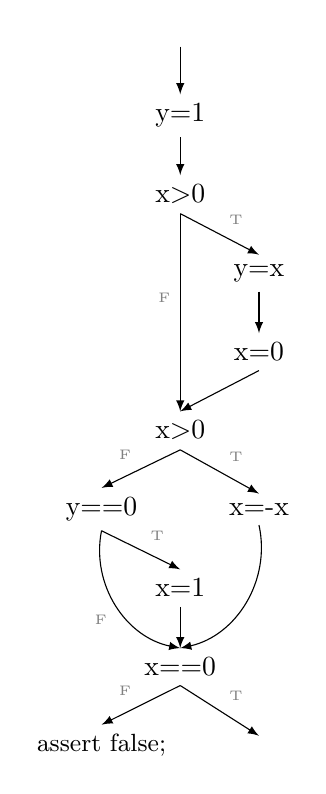
\begin{tikzpicture}[>=latex]
\node[name=enter]{};
\node[name=stmt_1, below of=enter]{y=1};
\node[name=if_1, below of=stmt_1]{x$>$0};
\node[name=if_1_body_1, below of=if_1, xshift=10mm]{y=x};
\node[name=if_1_body_2, below of=if_1_body_1]{x=0};
\node[name=if_2, below of=if_1_body_2, xshift=-10mm]{x$>$0};
\node[name=if_2_true, below of=if_2, xshift=10mm]{x=-x};
\node[name=if_3, below of=if_2, xshift=-10mm]{y==0};
\node[name=if_3_true, below of=if_3, xshift=10mm]{x=1};
\node[name=assert, below of=if_3_true]{x==0};
\node[name=exit, below of=assert, xshift=10mm] {};
\node[name=assertFalse, below of=assert, xshift=-10mm] {\small assert false;};

\draw(enter.south) edge[->](stmt_1.north);
\draw(stmt_1.south) edge[->](if_1.north);
\draw(if_1.south) edge[->]node[above right]{\tiny {\color{gray}T}}(if_1_body_1.north);
\draw(if_1_body_1.south) edge[->](if_1_body_2.north);
\draw(if_1_body_2.south) edge[->](if_2.north);
\draw(if_1.south) edge[->]node[above left]{\tiny {\color{gray}F}}(if_2.north);
\draw(if_2.south) edge[->]node[above right]{\tiny {\color{gray}T}}(if_2_true.north);
\draw(if_2.south) edge[->]node[above left]{\tiny {\color{gray}F}}(if_3.north);
\draw(if_3.south) edge[->]node[above right]{\tiny {\color{gray}T}}(if_3_true.north);
\draw(if_3_true.south) edge[->](assert.north);
\draw(if_3.south) edge[->, bend right=45]node[below left]{\tiny {\color{gray}F}}(assert.north);
\draw(if_2_true.south) edge[->, bend right=-45](assert.north);
\draw(assert.south) edge[->]node[above left]{\tiny {\color{gray}F}}(assertFalse.north);
\draw(assert.south) edge[->]node[above right]{\tiny {\color{gray}T}}(exit.north);

\end{tikzpicture}
\end{minipage}
\caption{Program example: source code and the corresponding CFG}
\label{fig:programExample}
\end{figure}

To verify the assertion we employ {\em zero} data-flow analysis whose abstract domain is defined by the set $\{\bot, 0, \neg 0, \top\}$. Where $\bot$ element represents the empty set of concrete values; $0$ -- the singleton set $\{0\}$ of concrete values, $\neg 0$ -- any concrete value except $0$ and $\top$ -- any concrete value. The left CFG on Figure~\ref{fig:analysisExample} shows the result of zero analysis where each edge is annotated with a tuple containing abstract values for x and y variables respectively. Clearly the analysis fails to verify $\varphi$ since it cannot prove that the false branch of x$==$0 condition is infeasible, i.e., the value of x or y is not $\bot$.

%How it can be more precise when it is changed to conditional.\\
One of the main reasons why data-flow analysis fails to verify $\varphi$ is the over-approximation that takes place when variable values from different paths are merged. For example, before the merge point the value of x on the true branch of $b_1$ is $0$ which is safely over-approximated by $\top$ at the merge point with the false branch of $b_1$. Thus, to improve the precision of data-flow analysis we need to restrict the set of paths it analyzes. It can be done by either restricting entry values of variables or by explicitly specifying the set of paths to be analyzed. We refer to the former as predicate-based condition and the latter as path-based condition.

%Now consider a case when the analysis has restricted the input domain of x to $0$ value. Then as shown on the middle left of Figure~\ref{fig:analysisExample} the analysis was able to determine that the assertion is not violated under that condition. Thus conditional analysis with the constraint $\phi :=$ x=$0 \land$ y = $\top$ are able to verify the program.

To illustrate conditional data-flow analysis with predicate-based we use the previous zero analysis and restrict the entry value of x  to the abstract domain element $0$. The result of such conditional analysis is shown on middle left CFG of Figure~\ref{fig:analysisExample}. The picture shows that condition was able to increase the precision of zero analysis since the analysis was able to verify the program for the entry value x$=0$.

Obviously in order to make the verification unconditional the analysis must also show that $\varphi$ also holds for the condition complement, i.e., when they entry value of x is $\neg 0$. The middle right CFG that on the same figure shows that as in the case of the original analysis the result is inconclusive. Thus conditions expressed as predicates over the input values not necessarily improve data-flow analysis precision.

To illustrate conditional data-flow analysis with path-based condition we restrict zero analysis to propagate program facts along the true branch of $b_1$ while skipping its false branch. The right CFG on Figure~\ref{fig:analysisExample} depicts the result of such conditional analysis. Once again conditional zero analysis was able to determine that all program paths following the true outcome of $b_1$ do not violate $\varphi$. Yet when the analysis is restricted to only the false branch of $b_1$ the result becomes inconclusive again.

\begin{figure*}[t]
\begin{minipage}{0.22\textwidth}
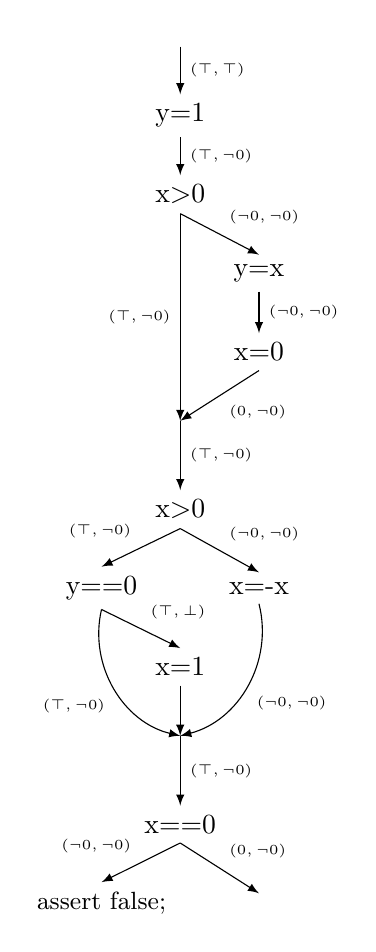
\begin{tikzpicture}[>=latex]
\node[name=enter]{};
\node[name=stmt_1, below of=enter]{y=1};
\node[name=if_1, below of=stmt_1]{x$>$0};
\node[name=if_1_body_1, below of=if_1, xshift=10mm]{y=x};
\node[name=if_1_body_2, below of=if_1_body_1]{x=0};
\node[name=if_1_merge, below of=if_1_body_2, xshift=-10mm]{};
\node[name=if_2, below of=if_1_merge]{x$>$0};
\node[name=if_2_true, below of=if_2, xshift=10mm]{x=-x};
\node[name=if_3, below of=if_2, xshift=-10mm]{y==0};
\node[name=if_3_true, below of=if_3, xshift=10mm]{x=1};
\node[name=if_2_merge, below of=if_3_true]{};
\node[name=assert, below of=if_2_merge]{x==0};
\node[name=exit, below of=assert, xshift=10mm] {};
\node[name=assertFalse, below of=assert, xshift=-10mm] {\small assert false;};

\draw(enter.south) edge[->]node[right]{\tiny $(\top,\top)$}(stmt_1.north);
\draw(stmt_1.south) edge[->]node[right]{\tiny $(\top,\neg 0)$}(if_1.north);
\draw(if_1.south) edge[->]node[above right]{\tiny $(\neg 0, \neg 0)$}(if_1_body_1.north);
\draw(if_1_body_1.south) edge[->]node[right]{\tiny $(\neg 0,\neg 0)$}(if_1_body_2.north);
\draw(if_1_body_2.south) edge[->]node[below right]{\tiny $(0,\neg 0)$}(if_1_merge.north);
\draw(if_1.south) edge[->]node[left]{\tiny $(\top,\neg 0)$}(if_1_merge.north);
\draw(if_1_merge.north) edge[->]node[right]{\tiny $(\top, \neg 0)$}(if_2.north);
\draw(if_2.south) edge[->]node[above right]{\tiny $(\neg 0, \neg 0)$}(if_2_true.north);
\draw(if_2.south) edge[->]node[above left]{\tiny $(\top,\neg 0)$}(if_3.north);
\draw(if_3.south) edge[->]node[above right]{\tiny $(\top, \bot)$}(if_3_true.north);
\draw(if_3_true.south) edge[->](if_2_merge.north);
\draw(if_3.south) edge[->, bend right=45]node[below left]{\tiny $(\top, \neg 0)$}(if_2_merge.north);
\draw(if_2_true.south) edge[->, bend right=-45]node[below right]{\tiny $(\neg 0, \neg 0)$}(if_2_merge.north);
\draw(if_2_merge.north) edge[->]node[right]{\tiny $(\top,\neg 0)$}(assert.north);
\draw(assert.south) edge[->]node[above left]{\tiny $(\neg 0, \neg 0)$}(assertFalse.north);
\draw(assert.south) edge[->]node[above right]{\tiny $(0, \neg 0)$}(exit.north);
\end{tikzpicture}
\end{minipage}
~
\begin{minipage}{0.22\textwidth}
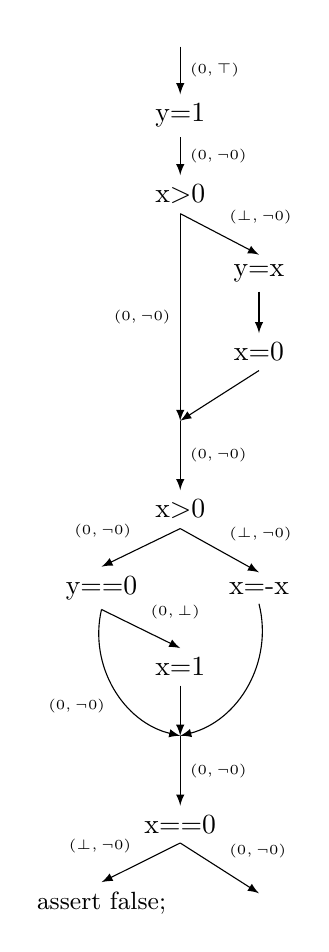
\begin{tikzpicture}[>=latex]
\node[name=enter]{};
\node[name=stmt_1, below of=enter]{y=1};
\node[name=if_1, below of=stmt_1]{x$>$0};
\node[name=if_1_body_1, below of=if_1, xshift=10mm]{y=x};
\node[name=if_1_body_2, below of=if_1_body_1]{x=0};
\node[name=if_1_merge, below of=if_1_body_2, xshift=-10mm]{};
\node[name=if_2, below of=if_1_merge]{x$>$0};
\node[name=if_2_true, below of=if_2, xshift=10mm]{x=-x};
\node[name=if_3, below of=if_2, xshift=-10mm]{y==0};
\node[name=if_3_true, below of=if_3, xshift=10mm]{x=1};
\node[name=if_2_merge, below of=if_3_true]{};
\node[name=assert, below of=if_2_merge]{x==0};
\node[name=exit, below of=assert, xshift=10mm] {};
\node[name=assertFalse, below of=assert, xshift=-10mm] {\small assert false;};

\draw(enter.south) edge[->]node[right]{\tiny $(0,\top)$}(stmt_1.north);
\draw(stmt_1.south) edge[->]node[right]{\tiny $(0,\neg 0)$}(if_1.north);
\draw(if_1.south) edge[->]node[above right]{\tiny $(\bot, \neg 0)$}(if_1_body_1.north);
\draw(if_1_body_1.south) edge[->](if_1_body_2.north);
\draw(if_1_body_2.south) edge[->](if_1_merge.north);
\draw(if_1.south) edge[->]node[left]{\tiny $(0,\neg 0)$}(if_1_merge.north);
\draw(if_1_merge.north) edge[->]node[right]{\tiny $(0, \neg 0)$}(if_2.north);
\draw(if_2.south) edge[->]node[above right]{\tiny $(\bot, \neg 0)$}(if_2_true.north);
\draw(if_2.south) edge[->]node[above left]{\tiny $(0,\neg 0)$}(if_3.north);
\draw(if_3.south) edge[->]node[above right]{\tiny $(0, \bot)$}(if_3_true.north);
\draw(if_3_true.south) edge[->](if_2_merge.north);
\draw(if_3.south) edge[->, bend right=45]node[below left]{\tiny $(0, \neg 0)$}(if_2_merge.north);
\draw(if_2_true.south) edge[->, bend right=-45](if_2_merge.north);
\draw(if_2_merge.north) edge[->]node[right]{\tiny $(0,\neg 0)$}(assert.north);
\draw(assert.south) edge[->]node[above left]{\tiny $(\bot, \neg 0)$}(assertFalse.north);
\draw(assert.south) edge[->]node[above right]{\tiny $(0, \neg 0)$}(exit.north);
\end{tikzpicture}
\end{minipage}
~
\begin{minipage}{0.22\textwidth}
\begin{tikzpicture}[>=latex]
\node[name=enter]{};
\node[name=stmt_1, below of=enter]{y=1};
\node[name=if_1, below of=stmt_1]{x$>$0};
\node[name=if_1_body_1, below of=if_1, xshift=10mm]{y=x};
\node[name=if_1_body_2, below of=if_1_body_1]{x=0};
\node[name=if_1_merge, below of=if_1_body_2, xshift=-10mm]{};
\node[name=if_2, below of=if_1_merge]{x$>$0};
\node[name=if_2_true, below of=if_2, xshift=10mm]{};
\node[name=if_3, below of=if_2, xshift=-10mm]{{\em the rest is the same }};
\node[name=if_3_true, below of=if_3, xshift=10mm]{{\em as on the leftmost graph}};
\node[name=if_2_merge, below of=if_3_true]{};
\node[name=assert, below of=if_2_merge]{};
\node[name=exit, below of=assert, xshift=10mm] {};
\node[name=assertFalse, below of=assert, xshift=-10mm] {};

\draw(enter.south) edge[->]node[right]{\tiny $(\neg 0,\top)$}(stmt_1.north);
\draw(stmt_1.south) edge[->]node[right]{\tiny $(\neg 0,\neg 0)$}(if_1.north);
\draw(if_1.south) edge[->]node[above right]{\tiny $(\neg 0, \neg 0)$}(if_1_body_1.north);
\draw(if_1_body_1.south) edge[->]node[right]{\tiny $(\neg 0, \neg 0)$}(if_1_body_2.north);
\draw(if_1_body_2.south) edge[->]node[below right]{\tiny $(0, \neg 0)$}(if_1_merge.north);
\draw(if_1.south) edge[->]node[left]{\tiny $(\neg 0,\neg 0)$}(if_1_merge.north);
\draw(if_1_merge.north) edge[->]node[right]{\tiny $(\top, \neg 0)$}(if_2.north);

\end{tikzpicture}
\end{minipage}
~
\begin{minipage}{0.22\textwidth}
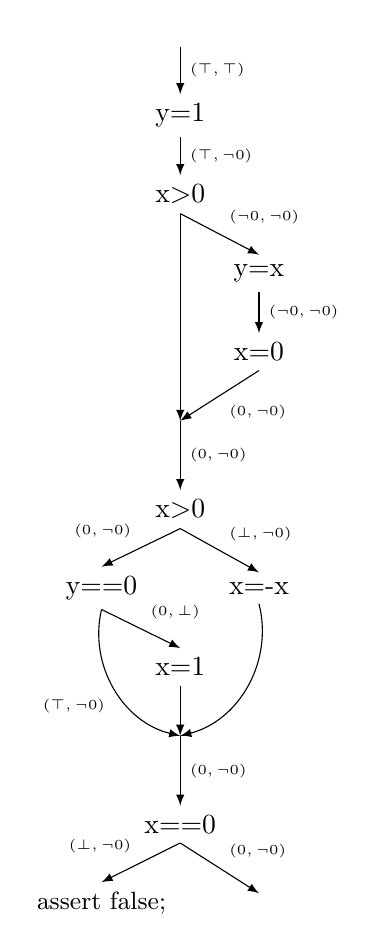
\begin{tikzpicture}[>=latex]
\node[name=enter]{};
\node[name=stmt_1, below of=enter]{y=1};
\node[name=if_1, below of=stmt_1]{x$>$0};
\node[name=if_1_body_1, below of=if_1, xshift=10mm]{y=x};
\node[name=if_1_body_2, below of=if_1_body_1]{x=0};
\node[name=if_1_merge, below of=if_1_body_2, xshift=-10mm]{};
\node[name=if_2, below of=if_1_merge]{x$>$0};
\node[name=if_2_true, below of=if_2, xshift=10mm]{x=-x};
\node[name=if_3, below of=if_2, xshift=-10mm]{y==0};
\node[name=if_3_true, below of=if_3, xshift=10mm]{x=1};
\node[name=if_2_merge, below of=if_3_true]{};
\node[name=assert, below of=if_2_merge]{x==0};
\node[name=exit, below of=assert, xshift=10mm] {};
\node[name=assertFalse, below of=assert, xshift=-10mm] {\small assert false;};

\draw(enter.south) edge[->]node[right]{\tiny $(\top,\top)$}(stmt_1.north);
\draw(stmt_1.south) edge[->]node[right]{\tiny $(\top,\neg 0)$}(if_1.north);
\draw(if_1.south) edge[->]node[above right]{\tiny $(\neg 0, \neg 0)$}(if_1_body_1.north);
\draw(if_1_body_1.south) edge[->]node[right]{\tiny $(\neg 0,\neg 0)$}(if_1_body_2.north);
\draw(if_1_body_2.south) edge[->]node[below right]{\tiny $(0,\neg 0)$}(if_1_merge.north);
\draw(if_1.south) edge[->](if_1_merge.north);
\draw(if_1_merge.north) edge[->]node[right]{\tiny $(0, \neg 0)$}(if_2.north);
\draw(if_2.south) edge[->]node[above right]{\tiny $(\bot, \neg 0)$}(if_2_true.north);
\draw(if_2.south) edge[->]node[above left]{\tiny $(0,\neg 0)$}(if_3.north);
\draw(if_3.south) edge[->]node[above right]{\tiny $(0, \bot)$}(if_3_true.north);
\draw(if_3_true.south) edge[->](if_2_merge.north);
\draw(if_3.south) edge[->, bend right=45]node[below left]{\tiny $(\top, \neg 0)$}(if_2_merge.north);
\draw(if_2_true.south) edge[->, bend right=-45](if_2_merge.north);
\draw(if_2_merge.north) edge[->]node[right]{\tiny $(0,\neg 0)$}(assert.north);
\draw(assert.south) edge[->]node[above left]{\tiny $(\bot, \neg 0)$}(assertFalse.north);
\draw(assert.south) edge[->]node[above right]{\tiny $(0, \neg 0)$}(exit.north);
\end{tikzpicture}
\end{minipage}
\caption{Analysis examples: {\em zero} analysis result (left), conditional {\em zero} analysis result with restricted input domain $x=0$ (middle left), $x=\neg 0$ (middle right), and the restricted set of paths (right).} 
\label{fig:analysisExample}
\end{figure*}

These examples indicate that some predicate and path based conditions posed on data-flow analysis can improve its precision. However, unlike previous work where conditions enabling the best precision can either be determined from the analysis design or during analysis run, for data-flow analysis such conditions cannot be obtained  using methods described in the related work. The section on related work describes in details the reason but in the essence the cause is that data-flow analysis cannot distinguish the source of precision losses which can be due to the over-approximation or due to the analysis design.

Thus the purpose of our work is to investigate what type of conditions, i.e., predicate-based, path-based or their combination, is better fitted to improve the precision of data-flow analysis. In order to obtain a better evaluation we not only compare condition types based on their ability to enable the best precision (like on the middle left and right CFGs of Figure~\ref{fig:analysisExample}) but also based their partial result, i.e., when an analysis can verify $\varphi$ on a subset of analyzed paths. As example consider the original zero analysis on left of Figure~\ref{fig:analysisExample}. Even though the analysis cannot verify $\varphi$ for all paths it can definitely tell that the set of paths containing the true branch of $b_3$ cannot violate $\varphi$ because these paths are infeasible. To represent and compare partial results of conditional data-flow analysis we introduce path language. Using such encoding we can record the partial result of unconditional zero analysis as $*;b_3;*$ and the result of condition zero analysis on the rightmost CFG of Figure~\ref{fig:analysisExample} as $b_1;*$. Section ... explores the paths language in greater details.

Overall our work focuses on answering (empirically) the following research questions:
\begin{enumerate}
\item Does the predicate-based precondition increase the partial output of data-flow analysis?
\item Does the path-based precondition increase the partial output of data-flow analysis?
\item How do the two representations compare with each other?
\item Does the combination of predicate-based and path-based preconditions increase the partial output of data-flow analysis comparing to their separate results.
\end{enumerate}

%Why we cannot determine a priori or during run-time what is needed for a better precision. And why it can be done for model checker and why model checker can always produce answer for the given set of path and why logical characterization is sufficient for it. But the logical characterization is not possible for d.f.a. Because in conditional model checking the predicates are tracked.

%A key here is to crystalize the contributions of the work, e.g., data flow analysis
%\begin{itemize}
%\item requires a new means of encoding conditions -- path languages;
%\item introduces overapproximation when it encounters program structures that are a mismatch for its reasoning engine which makes triggering condition generation more challenging, whereas verification approaches can detect those mismatches syntactically;
%\item something about ``partial analysis results''
%\end{itemize}





\section{Formalizing Conditional Analyses}
\label{section:formalizing}
%reuse as much technical machinery from Conway as makes sense

%we want to include as much analytical content as possible, since
%this reduces the expectation for empirical evaluation.  Specifically
%we want to discuss
%\begin{itemize}
%\item prove that state-specific conditions are insufficient to express
%input-related conditions, but that input-related conditions are sufficient
%\item define the conditions under which path and predicate encodings are
%equivalen
%\item anything else that makes sense
%\end{itemize}
Similarly to the previous section in this section we first present the traditional monotone framework for data flow analysis followed by the discussion of the necessary changes that extend it to a conditional data flow framework. This section also outlines the approach of composing the unconditional result from conditional ones.

We use the data flow analysis framework as presented in~\cite{Nielson:1999} where an analysis $\mathcal{A}$ is defined by the following parameters. 
\begin{itemize}
\item The complete lattice $D_\mathcal{A}$ that describes the abstract domain of $\mathcal{A}$.
\item $CFG_P$ for a program $P$.
\item  A set of monotone transfer functions $\mathcal{F}_\mathcal{A}$ for each statement $l \in CFG_P$ that maps an element of $D_\mathcal{A}$ to itself, i.e., $f_l \in \mathcal{F}_\mathcal{A} : D_\mathcal{A} \mapsto D_\mathcal{A}$.
\item Entry statements $E$ in $CFG_P$.
\item An initial value $\iota\in D_\mathcal{A}$ for statements in $E$.
\end{itemize}

Then the set of equations for forward $\mathcal{A}$ is defined as follows on entry and exit of each statement $l\in CFG_P$:
\begin{eqnarray*}
\mathcal{A}_{in}(l) &= &\bigsqcup\{\mathcal{A}_{out}(l') \;|\; (l',l)\in CFG_P\}\sqcup \iota_E^l\\
 &  & \text{ where } \iota_E^l = \left\{ \begin{array}{rl}
 \iota &\mbox{ if $l\in E$} \\
  \bot &\mbox{ if $l\not\in E$}
       \end{array}\right. \\
\mathcal{A}_{out}(l) & = & f_l(\mathcal{A}_{in}(l))     
\end{eqnarray*}
where $\sqcup$ is the least upper bound operator, $\bot$ is the bottom element of $D_{\mathcal{A}}$ for which $\forall d\in D_\mathcal{A} : \bot\sqcup d = d$ and $\forall l\in CFG_P :  f_l(\bot)=\bot$. For the safety properties $\bot$ corresponds to the empty set of concrete values and $\top$ to the set containing all concrete values. The value of $\iota$ is assigned to $\top$, i.e., the analysis considers all possible input values for a program. The solution of the above set of equations provides is the result of the analysis for $P$.

Recall that a condition for data flow analysis can be expressed as a predicate $\phi$ over the input values or as $\pi$ -- condition that identifies the set of paths to be analyzed. Since $\phi$ and $\pi$ are incomparable the overall condition $\theta$ for a conditional data flow analysis $\mathcal{A}^\theta$ is described by a tuple of $\phi$ and $\pi$, i.e., $\mathcal{A}^{(\phi,\pi)}$.

%We express $\pi$ as a regular language with the alphabet $\Sigma_\pi$  over branch outcomes of conditional statements $b_l$. We refer to it as {\em path language}. If $b_l$ has $l'$ and $l''$ its true and false targets, respectively then the symbols $S_\pi\subset \Sigma_\pi$ of the regular expression representing $\pi$ can contain $(b_l,l')$, or $(b_l,l'')$, or none of them. Also we require that $S_\pi$ appear in $\pi$ in their topological ordering of $CFG_P$. Thus $\pi = .^*;(b_l,l');.^*$ describes a set of paths that execute the true branch of $b_l$. In this case when $\mathcal{A}^{(\phi,\pi)}$ encounters $b_l$ on the false edge $(b_l, l'')$ it sets the variable values incoming to $l''$ to $\bot$. For brevity  we denote the case when $\forall i : x_i = \bot$ as $\bot$.  When none of the edges are present in $\pi$ then the analysis treats them in its usual manner, i.e., propagates the information through both branches. 

We have chosen $\pi$ to be represented by the set of branch edges in $CFG_P$, at most one for each conditional statement $l$,  which the analysis must include while excluding their counterparts. If $l$ has $l'$ and $l''$ as its true and false targets, respectively, then $\pi$ can contain  the edge $(l,l')$, or the edge $(l,l'')$, or none of them. To capture the relation between the opposite branches of $l$ we designate $(l,l')=\neg (l,l'')$ and the vice versa $(l,l'') = \neg (l,l')$. If $(l,l') \in \pi$ then the values of all variables $x_i$ incoming to the target  of its opposite edge $l''$, i.e., along edge $\neg (l,l')$, will be set to $\bot$. For brevity  we denote such case, i.e., when $\forall i : x_i = \bot$, as $\bot$ state.The same principle applies when $(l,l'') \in \pi$.   When none of the edges are present in $\pi$ then the analysis treats them in its usual manner, i.e., propagates the information through both branches.

For a set of input variables $x_i$ $\phi$ can be represented as an assignment of $x_i$ to its initial values from $d_i \in D_\mathcal{A}\setminus\{\bot\}$. In the traditional data flow analysis all $x_i$ are set to $\top$ element of  $D_\mathcal{A}$. For shortness we refer to such condition as $\top$.

Thus a traditional data flow analysis $\mathcal{A} = \mathcal{A}^{(\top,\emptyset)}$, for a conditional analysis with predicate-based condition $\mathcal{A}^{(\phi,\emptyset)}$ and so on. In the related work on the conditional model checking a condition $\theta$ also consists of two parts. In the case when a model checker runs out of resources it outputs the set of predicates describing analyzed paths, which is equivalent to $\phi$ predicate-based condition. In the case when a model checker cannot reason about some set of paths it records them in a structural way which is similar to $\pi$ path-based condition.

%We have two type of constraints name it $\phi$ and $\pi$ which describe the restriction on the initial conditions (note that it is different from $\mathcal{I}$ and $\pi$ describes the set of branches of conditional statement to exclude form the execution. This type of composition is also present in the related work. The idea in conditional model checking is that $\phi$ is used when an analysis able to reason about the set of path it analyzed but run out of resources and the structural description when it cannot crate such description thus an universal description is taken. (See also reasoning below).

%In conditional model checking the condition $\theta$ for which the results holds consists of two parts. When a model checker runs out of resources it describes the part of the state space it has been analyzed as logical formula over predicates, we call it $\phi$. But, when the model checker encounters a conditional statement it cannot reason about then obviously it is unable to express the path containing that predicate as a logical formula anymore. Instead it uses a structural, i.e., CFG path-based, description of that path. Thus for an arbitrary of conditional model checker the condition $\theta$ consists of two parts: $\phi$ -- the predicate-based encoding of covered input state space and $\pi$ -- the path-based encoding of the assumed paths.

%Similarly a condition of data flow analysis can also have such dual representation. In that case predicate-based condition $\phi$ describes the part input state space that is analyzed. Alternatively the input state space can be represented as the set of paths $\Pi$ in the program's CFG. This way a set of paths $\pi$ is also described a part of the program's input space but expressed structurally. In conditional model-checking $\phi$ can be expressed through $\pi$ since model checking is a MOP analysis. However, such correspondence does not exist in data-flow analysis. Thus conditions expressed by $\phi$ and $\pi$ are incomparable analytically in data flow analysis. Therefore in order to formalize conditional data flow analysis we employ both $\phi$ and $\pi$ parts of $\theta$.

With the proposed above predicate and path based conditions we can now write the set of equations for conditional data flow framework for an analysis $\mathcal{A}^{(\phi,\pi)}=\mathcal{A}^\theta$:

\begin{eqnarray*}
\mathcal{A}_{in}^{\theta}(l) &= &\bigsqcup\{\mathcal{A}_{out}^{\theta}(l') \;|\; (l',l)\in CFG_P, \neg(l',l) \not\in\pi\}\sqcup \iota_E^l\\
 &  & \text{ where } \iota_E^l = \left\{ \begin{array}{rl}
 \phi &\mbox{ if $l\in E$} \\
  \bot &\mbox{ if $l\not\in E$}
       \end{array}\right. \\
\mathcal{A}_{out}^{\theta}(l) & = & f_l(\mathcal{A}_{in}^{\theta}(l))     
\end{eqnarray*}
where for the first equation we assume $\forall d\in D_{\mathcal{A}} : \emptyset\sqcup d =  d$.

Let $\Phi$ and $\Pi$ be the universe of predicate-based and path-based conditions, respectively, for an analysis $\mathcal{A}$. Executing $\mathcal{A}$ with different conditions $\phi_i\in \Phi$ and $\pi_j\in\Pi$ produces a set of conditional analysis $\mathcal{A}^{(\phi_i,\pi_j)}$. Having these conditional analysis we would like to determine whether its combined effort produces the result of the unconditional analysis. To answer this question we first identify the method for combining conditions $(\phi_i,\pi_j)$ for the same $\mathcal{A}$ and then establish the requirement when combined conditions imply the unconditional result.

Consider two conditions $(\top,\{(l,l')\})$ and $(\top,\{\neg(l,l')\})$. The conditional analysis $\mathcal{A}^{(\top,\{(l,l')\})}$ analyzes all possible input values for the set of paths containing the true branch of $l$ while $\mathcal{A}^{(\top,\{\neg(l,l')\})}$ does it for the set of paths containing the false branch of $l$. Obviously, the cumulative result of $\mathcal{A}^{(\top,\{(l,l')\})}$ and $\mathcal{A}^{(\top,\{\neg(l,l')\})}$ is unconditional. To automate the process of combining the set of paths we convert $\pi$ into a boolean function $g_\pi$ as follows.  Each true edge in $CFG_P$ is mapped to a boolean variable $x_i$ and each false edge is mapped to $\neg x_i$. Then edges in $\pi$ are mapped to a set of literals, i.e., variables and its negations, and $g_\pi$ is expressed as the conjunction of those literals. In our example if $(l,l')$ is mapped to $x_5$ then $g_{\{(ll')\}} := x_5$ and $g_{\{\neg(ll')\}} := \neg x_5$. The union of these two sets of paths is equivalent of the disjunctions of $g_{(ll')}$ and $g_{\neg(ll')}$. Thus the combination of arbitrary $\pi_1$ and $\pi_2$ is equivalent to 
$$
g_{\pi_1}\lor g_{\pi_2} \equiv \pi_1 \cup \pi_2 
$$

Combing two conditions with different predicate condition and the same paths like $(\phi_1, \pi)$ and $(\phi_2, \pi)$ is more straightforward. Since for input variables $x_i$ and $d_i\in D_{\mathcal{A}}$ 
$$\phi_1=(x_1=d_1,\dots, x_n=d_n)$$ and 
$$\phi_2=(x_1=d_{n+1},\dots, x_n=d_{2n})$$ 
then the combination of $\phi_1$ and $\phi_2$ is 
$$(x_1=d_1\sqcup d_{n+1},\dots, x_n=d_n\sqcup d_{2n}) \equiv \phi_1\sqcup \phi_2$$

The criterion for which the set of conditional analyses equivalent to unconditional result is when the combination of their conditions returns the tuple $(\top, true)$. To combine the set of conditions $\{(\phi_i,\pi_j)\}$ where $\phi_i\in \Phi$ and $\pi_j\in\Pi$ we first partition them into subsets with the same $\pi_j$ 
$$
\{(\phi_i,\pi_j)\} = \{(\phi_i, \pi_1)\}\cup\dots\cup \{(\phi_i, \pi_n)\} 
$$
and combine $\phi$ as described above
$$
\{\sqcup_i\{(\phi_i, \pi_1)\},\dots,\sqcup_i\{(\phi_i, \pi_n)\} \}= \{(\phi_{i_1},\pi_1),\dots,(\phi_{i_n},\pi_n)\}
$$
where $\phi_{i_j}\in\Phi$ and not necessary unique. Next we separate the result above into subsets with the same $\phi_{i_j}$
$$
\cup_j\{(\phi_1,\pi_j)\}\cup\dots\cup\cup_j\{(\phi_m,\pi_j)\}
$$
and union the paths in each partition by converting them to boolean functions $g_{\pi}$ and mapping them back to the set representation
$$
\{\lor_j\{(\phi_1,g_{\pi_j})\}, \dots, \lor_j\{(\phi_m,g_{\pi_j)}\}\} = \{(\phi_1,\pi_{j_1}),\dots,(\phi_m,\pi_{j_m})\}
$$
In the case when
$$
\{(\phi_1,\pi_{j_1}),\dots,(\phi_m,\pi_{j_m})\} = \{(\top,\emptyset)\}
$$
then the result is unconditional.

\section{Applications of Conditional Analysis}
\label{section:applications}
What Elena described about two programs and two analyses

If possible we should introduce the key research questions
early in the paper.  As I said earlier, if we can provide
partial answers to the questions via analytical argument
that is best.


\section{Related Work}
\label{section:Related}
In the introduction we have highlighted the key concepts presented in the previous publications on conditional analyses. In this section we describe most relevant to our work ideas from those papers. The earlier research has introduced two ``conditional'' notions -- {\em conditional soundness} and {\em conditional analysis}. In their essence both concepts are the same -- the result of an analysis holds only under the established conditions. They diverge in their approaches in obtaining unconditional results. Conditional soundness relies on another analysis to prove that the program states that satisfy the negated condition are not reachable, i.e., showing the infeasibility of the program execution containing those states. While conditional analysis may use the same or a different analysis to show that those states do not violate properties either by appearing in behaviors that conform to the properties or by belonging to  infeasible program executions.

The work on conditional soundness~\cite{Conway:SAS08} explores the dependency of the soundness of one analysis on the result of another analysis. Many analyses assume that a program is ``well-behaved'', for example an analysis with the abstract domain $\{-,0,+\}$ assumes the absence of overflow conditions when the rule $\{+\} + 1$ produces not expected $\{+\}$ but $\{-\}$. The authors demonstrate this concept on a pointer analysis for C program. A points-to analysis can produce sound results if the program is memory safe, i.e., there is no out of bound accesses. The authors argue that it is possible to combine points-to and memory safe analyses into a single analysis but such approach is not scalable. Thus they propose to first perform points-to analysis assuming that the program is memory safe and after that run the memory safety analysis with the points-to analysis result to prove that the assumption holds.

Besides explaining the concept of conditional soundness the authors also formalize it through a set of definitions. They specify of a conditional soundness with respect to a predicate $\theta$ on a concrete state. Then an analysis is defined to be $\theta$ sound when it over-approximates program behavior reachable through concrete states satisfying $\theta$. Thus an analysis applies its transfer function only to the states satisfying $\theta$. However, the transfer function can produce non-$\theta$ states but those states will not be explored on the next application of the transfer function.  In order to prove an unconditional soundness of the first analysis the second analysis explores the states produced by the first analysis and proves that resulted non-$\theta$ states are unreachable in the program.

The work~\cite{Naik:POPL07} on static race detection for multi-threaded programs is conceptually similar to the previously described paper on conditional soundness. A static race detection algorithm analyzes memory accesses $m_1$ and $m_2$ guarded by locks $l_1$ and $l_2$ respectively. It assumes that $m_1$ and $m_2$ may alias and thus the algorithm aims to prove that $l_1$ and $l_2$ must alias in order for a program to be race free. In the alternative approach proposed in this paper it is assumed that $l_1$ and $l_2$ must not alias and then it is shown that $m_1$ and $m_2$ cannot refer to the same memory location. The absence of aliasing between $m_1$ and $m_2$ is easy to show when $m_i$ is the field of the object referred by $l_i$ and that the field $m_i$ is only reachable through that object. However, in order to make the result of the analysis sound unconditionally another analysis must be prove that $l_1$ and $l_2$ in fact must not alias.

%The main goal of the conditional model checking approach is not to waste resources when a model checker cannot verify the whole program either because of its inability to handle assertion, i.e., not in that domain or running out of resources.
The authors of the paper on conditional model checking~\cite{Beyer:Tech11} emphasize the fact that when a model checker fails either to verify a program or to produce a counterexample then the effort put into the exploration of the program's state space is wasted. These situations arise when either the model checker runs out of computational resources or its unable to decide on the predicate of a branch condition. The latter takes place when the model checker is not designed to handle the theory used in the predicate, e.g., the predicate analysis cannot handle non-linear arithmetic.

In the case of resources exhaustion, i.e., either running out of memory or timing out,  instead of conventional termination the authors propose an informative termination where upon shutting down the model checker produces data that describes the parts of the state space it was able to verify. To characterize the parts of the analyzed state space the model checker enhances each abstract state with a predicate that uniquely describes that state. Hence, when the model checker depletes its computational resources, instead of terminating with a run-time exception, it returns a condition describing the set of states it has analyzed. The condition is expressed as a conjunction of the analyzed states predicates. The next model checker can use the negated condition to guide itself to the part of the state space that was not analyzed by the previous model checker. This characteristic of conditional model checker corresponds to the notion of conditional analysis.

In the case of undecidable predicates the authors propose to proceed with such predicate interpretation that permits the model checker to proceed with the verification, e.g., assuming that an assertion it cannot reason about does hold. The encountered assumptions for taken branches are encoded as an automaton that is used to guide the further analysis to the assumed branches. These assumptions must be analyzed further by another model checker that is capable to reason about them. If the subsequent model checker determines that these assumptions hold then the verification is complete. This side of conditional model checker relates to the idea of conditional soundness.

%Moreover, this conditional approach allows a model checker to express its bounds like the tree depth, loop unrolling bounds and other boundary criteria as a condition. Thus if a model checker was not able to find  Also when a model checker is bounded by the depth of a path or location repetition the technique is able to translate these bounds into conditions which can describe for what states the model checker was able to verify the program.

A conditional model checker integrates assumptions, i.e., conditional soundness for certain states, and predicate , i.e., conditional analysis, information into the characteristic of abstract states. At the end of the execution  the conditional model checker traverses the reached abstract states and produces the condition and the branch outcome assumption information. The experiments presented in the paper have shown that applying conditional model checkers with feedback capabilities increased the number of verified programs.

%The fundamental difference with our approach is model checking is MOP analysis where each path is analyzed separately. Thus if an analysis cannot decide something is not because it lost information on a merge point, the analysis cannot handle it inherently like a non-linear arithmetic. In MOP one can specify additional bounds as loop unrolling, resource time out, depth of a search tree to be quantified as a condition.

%In MFP analysis one cannot have condition as loop unrolling (inapplicable), or timeout (not sound). In MFP imprecision may arise due to merging operator on control flows.

Our work differs from the previous research in the approach of determining the condition for which an analysis guarantees its most accurate result. In the work on conditional soundness these conditions are defined a priori and applied for all states, e.g., no integer overflows. These conditions are derived straight from the design of the analysis. Without those conditions in place the analysis is unable to produce a correct answer. A conditional model checker discovers the conditions, i.e., the assumptions, for its optimal result while analyzing a program. Although its conditions only applicable to some set of states, e.g., the false branch of the conditional statement on line 10 is infeasible. 

However, conditional data-flow analysis cannot use neither of these approaches. Clearly, finding the conditions solely from the design of data-flow analysis is not possible because these conditions are program dependent. Therefore no a priori conditions can be determined. Determining them during analysis run as done in the conditional model checking is also problematic. The reason is that model checking and data-flow analysis have different underlying analysis frameworks. Model checking is based on meet over path (MOP) analysis framework where an analysis calculates facts for each program path separately. While data flow analysis is based on maximal fixed point (MFP) analysis framework where only a single fact is calculated for a set of paths and that fact over-approximates the facts of the evaluated paths.

Thus, when an MOP analysis cannot decide on a branch outcome it is solely due to the analysis theory being inadequate. However, for an MFP analysis an imprecision may also be the result of the over-approximating several paths with diverse facts. But the MFP analysis might produce a better result if the set of paths it over-approximates is smaller with more uniform facts. The current work looks into exploring alternative methods in partitioning program paths to increase the precision of data flow analysis.  

%In our case $\theta$ can be describes the set of states reachable from the restricted input domain or lay on the selected set of paths. In our case it is conditional analysis not conditional soundness.

%Also it combines different conditions as assumptions, location monitoring, overflow monitoring. For assumption the condition is an expression, for other the condition for an infeasible path is ``false'' which exclude that path. Also track predicates for the case of resources exhausting which tells what paths have been covered.

%Similar to conditional model checking, conditional soundness gives the condition under which analyses are most precise. Without this condition the analysis cannot produce any result, i.e., always unknown, and with that condition the analysis is able to produce some result. Soundness here is more related to the precision. Once again this is different from our work where we do not know when DF are the most precise.

%Similar that the result produces by conditional and data-flow analysis are only sound within that condition. 

%In order to prove unconditional soundness some other analysis must prove that non-$\theta$ states are not feasible. In our work for unconditional soundness we need to prove that non-$\theta$ states do not violate properties which also include showing that some non-$\theta$ states are not feasible.

%Work on the conditional model checking the unconditional soundness of the program is achieved as a hybrid. For assumption it is to show that non-$\theta_{assumption}$ states are not feasible and for partial result is to show that non-$\theta_{predicate}$ do not violate that condition. We just need to show the latter case. 

















\section{Conclusion and Future Work}
\label{section:conclusion}
\input{conclusion}

\section*{Acknowledgment}
The authors would like to thank...

\bibliographystyle{IEEEtran}
\bibliography{paper}

\end{document}


